\end{multicols}
\chapter{Theory}
\begin{multicols}{2}

\noindent A deeper understanding of all relevant aspects of the thesis problem
is laid out below.  Some references are made without being explained further;
these are to be considered as lying outside the delimitations of the thesis.

\section{Financial Markets}

A financial market is a trading market in which people trade financial
securities, commodities and other assets.  A market participant places a bid or
ask for a certain security; a binding commitment to buy or sell that security.
All current asks and bids are kept track of through the use of the \textit{order
  book}.  When a matching bid or ask is placed for the same security, a
\textit{transaction} occurs---the asset changes ownership to the purchasing
party (having placed a bid for the security) and money is transferred to the
selling party (having placed an ask for the security).

The number of asks and bids in the market at any point in time for a given price
level comprises the market \textit{depth}, and the total number of
\textit{transactions} (i.e.\ matching pairs of asks and bids) comprise the
traded \textit{volume} in the market (as opposed to the number of contracts in
the market; the \textit{market volume}).

Both bids and asks can be placed as \textit{market orders}, meaning that they
immediately trade at the current best market price (not counting slippage
costs).  The alternative is to specify a certain price---the limit
price---guaranteeing that the order will trade at a price no worse than the
limit price, hence sacrificing immediacy for certainty in regard to the
execution price (although the order risks not trading at all if the market never
reaches the limit price).  In fact, it is these, so called, limit orders that
show up in the limit order book.

Transactions also carry transaction costs, including a \textit{brokerage
  fee}---a fee charged by the broker to conduct transactions between buyers and
sellers, as well as an \textit{exchange fee}.

\subsection{The Foreign Exchange Market}

The Foreign Exchange Market (\textsc{forex}) is a global decentralized financial
market where currency pairs are traded.  Although it is a financial market like
many others, it has a certain set of attributes distinguishing it from others:
Its traded volume is the largest of any financial market, it is a global,
decentralized market, operated by a broker-dealer, as opposed to the more common
centralized exchanges (except for e.g.\ \textsc{forex} derivatives traded on the
\textsc{cme}), it is the most liquid asset of all asset classes, it is always
open (except weekends), price movements are generally very small and
broker-dealers offer highly leveraged margin accounts.

Market movements are announced as price interest points---\textit{pips} (on
other financial markets, known as \textit{ticks}). A pip designates a minimal
change in price.  For example, a price movement from $1.2345$ to $1.2346$
represents a single pip, i.e.\ a tick step of $0.0001$.  A pip is always a
change in the last decimal digit of the price (the currency exchange rate).

\subsection{Technical Analysis}

\textit{Technical} analysis of financial assets is a method for understanding
the asset value (and its movements) only by looking at previous market data
(i.e.\ volume, ask price, bid price etc.).  This can be looked at in contrast to
\textit{fundamental} analysis; estimating the intrinsic value of an asset by
looking at various aspects and properties of the underlying company, market
sector and macroeconomic factors; for example, looking at company financials or
social trends.

In regard to the efficient-market hypothesis---the hypothesis that the market is
efficient to such a degree that the market price immediately incorporates and
reflects all relevant information \citep{fama1995random}---the effectiveness of
technical analysis is disputed: The quote ``I realized that technical analysis
didn't work when I turned the chart upside down and didn't get a different
answer'' has been attributed to Warren Buffett, who prefers a fundamental
analysis approach to investment.  However, the overwhelming empirical evidence
of market inefficiencies suggests that the efficient market hypothesis can be
refuted, hence providing a solid foundation for predicting future market
behavior.

\subsection{Japanese Candlesticks}

Often a vital part in charting analysis, the Japanese candlestick provides a
simple method of aggregating and plotting market behavior \citep{nison2001}.
Instead of plotting each individual pip (resulting in a very flat and
\textit{very} wide chart), pips are aggregated into \textit{candlesticks}.  This
method can be used with any time frame (dictating how many pips end up in a
single candlestick).

The candlestick is made up of three parts: The real body, the upper shadow and
the lower shadow.  The real body is bounded by open and close prices for all
pips in the time frame aggregated into the candlestick.  For example, if the
time frame is one minute, assuming that the last pip has a higher value than the
first pip, the lower edge of the real body denotes the first pip encountered
that minute (the \textit{open price}), while the upper edge of the real body
denotes the \textit{last} pip during that minute (the \textit{close price}).
Otherwise, if the last pip has a lower value than the first pip, the lower edge
denotes the last pip, and the upper edge denotes the first pip. Usually,
candlesticks with a close price higher than open price are represented by a
white (sometimes green) body while candlesticks with a close price lower than an
open price are represented by a black (sometimes red) body.

The top of the upper shadow, positioned on top of the real body, represents the
\textit{high price} during that minute; the highest value encountered in any pip
that occurred during the time interval that the candlestick represents.
Likewise, the bottom of the lower shadow represents the \textit{low price}; the
lowest value found in any pip during the time frame.

Together, these provide the open, high, low and close prices during the
candlestick's time frame (often referred to as \textsc{ohlc} data.)

\begin{Figure}
  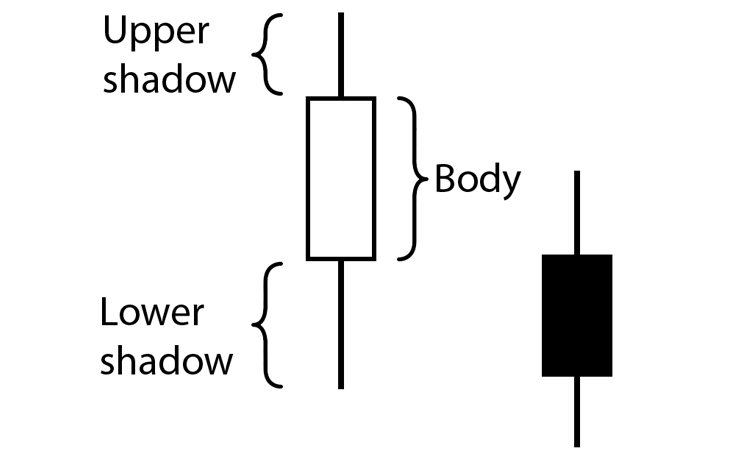
\includegraphics[width=\linewidth]{figures/candlestick}
  \captionof{figure}{The Japanese candlestick and its parts.}
\end{Figure}

\noindent Chart patterns (see below) often rely on Japanese candlestick
aggregation to provide meaningful indications regarding market behavior.
Moreover, the time frame represented by the candlestick can be set to any amount
of time, allowing the trader to perform the charting analysis using various
resolutions.

\subsection{Chart Patterns}

Giving more credibility to the idea of technical analysis, there exist certain
\textit{chart patterns} that can be observed prior to specific market
expectations and behavior \citep{technicalanalysis2010}. The patterns can bee
seen in the price movements of a financial security (sometimes combined with
looking at the market volume or any other aspect of market behavior).  As a
concrete example of a pattern, there is the \textit{bull flag}, represented by a
strong upwards movement (in the case of the bull flag, called the flagpole,
usually combined with a surge in market volume), after which a trend channel
(representing the flag) is charted.  When the price breaks through the upper
boundary of the trend channel, the bull flag pattern is completed and a
continuation of the rise is expected to follow.

There is also the \textit{double top} chart pattern (illustrated below), which
is a bearish reversal pattern; the pattern can be identified as two distinct
price tops reaching roughly the same level.  If the price of the financial
security drops below a certain lower boundary of a trend channel charted around
the pattern, it is expected that the price will drop further afterwards.

\begin{Figure}
  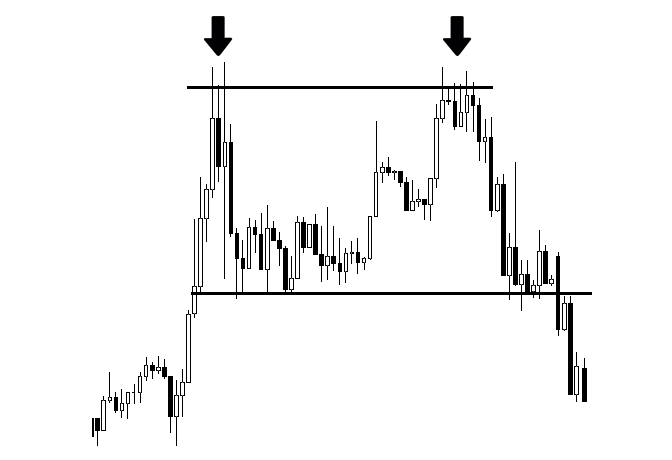
\includegraphics[width=\linewidth]{figures/double-top}
  \captionof{figure}{The bearish trend-reversal double top chart pattern.}
\end{Figure}

\noindent There are a several different chart patterns indicating and predicting
certain market behavior.  They raise an interesting and relevant point, which
will be touched upon again when the intricacies of neural network models are
discussed below: If there are certain patterns recurring before certain market
behavior, hypothetically, a properly configured neural network model should be
able to learn to identify them under the proper circumstances and thus show
potential in predicting market behavior.

These chart patterns are of great importance to the thesis problems, as---which
will be detailed in the machine learning section---recurring chart patterns is a
vital component for machine learning algorithms to model problems well.

No matter whether the trader is a human or a machine, chart patterns are a vital
part of a technical analysis approach to trading strategies. For the sake of the
thesis problem, we ascribe a high level of credibility to these chart
patterns---it is not part of this thesis to investigate their validity in
technical analysis trading.

\subsection{Technical Indicators}

While the occurrence of chart patterns are used as indicators for trading in
technical analysis, there are also other technical indicators in the form of
certain measures and computations of market properties.

As part of the trading strategy, like chart patterns, these technical
\textit{indicators} are used to aid in trading decisions.  All of the technical
indicators are based on already-available market information embedded in
e.g.\ prices, volume etc.  The technical indicators are computed on this
information, giving evaluation measures that can be used to make certain aspects
of the market behavior more prominent.

\subsubsection{Simple Moving Average (\textsc{sma})}

The Simple Moving Average is one of the most basic indicators used for trading.
It is calculated by simply summing a certain number of price points (in
sequence) together and dividing it by the number of price points sampled.  For
example, to calculate the \textsc{sma} of a price at time $t$: Sample $N$ points
before $t$, add the prices together and divide the resulting value by $N$:

\begin{Figure}
  \begin{align*}
    \mathit{SMA^N}(t) = \frac{1}{N}\sum\limits_{i=0}^{N-1} \mathit{Price(t-i)}
  \end{align*}
  \captionof{eqn}{Simple moving average formula.}
\end{Figure}

\subsubsection{Relative Strength Index (\textsc{rsi})}

The Relative Strength Index is a technical indicator used to assess the strength
and weakness of a financial asset based on the closing prices over a certain
period of time.  The \textsc{rsi} measures the velocity and magnitude of price
movements, computing the momentum---the rate of average gain versus average loss
in prices over a certain period.

The period used to calculate the \textsc{rsi} is normally set to fourteen days,
but the period can also be arbitrarily chosen.

The \textsc{rsi} gives a value on a scale from 0 to 100, with low and high
values set at 30 and 70, respectively. It is reasoned that an \textsc{rsi}
indicator showing a value lower than 30 indicates that a financial asset is
oversold, where as a value higher than 70 indicates that it is overbought
\citep{wilder1978}.

Although the \textsc{rsi} is slightly more complex to calculate than the
\textsc{sma}, a variation of the \textsc{rsi}---called Cutler's
\textsc{rsi}---provides a simpler way of calculating it.  Cutler reasoned that
the original \textsc{rsi}, introduced by \citet{wilder1978}, using a
\textit{smoothed moving average}, provided very different results depending on
what data point (time) in the sequence at which computation started.  Because of
this, Cutler's \textsc{rsi} is instead based on the \textsc{sma}:\@

\begin{Figure}
  \begin{align*}
    D^N(t) & = \frac{1}{N}\sum\limits_{i=0}^{N-1} max(\mathit{Price(t-i-1)} -
                                                     \mathit{Price(t-i)}, 0) \\
    U^N(t) & = \frac{1}{N}\sum\limits_{i=0}^{N-1} max(\mathit{Price(t-i)} -
                                                     \mathit{Price(t-i-1)}, 0) \\
    \mathit{RS^N}(t) & = \frac{U^N(t)}{D^N(t)} \\
    \mathit{RSI^N}(t) & = 100 - \frac{100}{1 + \mathit{RS^N}(t)}
  \end{align*}
  \captionof{eqn}{Cutler's relative strength index formula.}
\end{Figure}

\noindent There are many more technical trading indicators.  All of them claim
to measure various aspects of the data, and some of them work together to
provide a useful indication.

\subsection{Financial Measurements}

\subsubsection{Bid-ask Spread}

Although not strictly a trading indicator, the spread (difference between the
best ask and best bid prices) is used as a model feature in our setup. It is a
measurement of the transaction cost associated with market orders and an
indicator for the liquidity of the market. The formula for the spread is
trivial:

\begin{Figure}
  \begin{align*}
    \mathit{Spread(t)} = \mathit{Ask_t} - \mathit{Bid_t}
  \end{align*}
  \captionof{eqn}{Bid-ask spread formula.}
\end{Figure}

\subsubsection{Sharpe Ratio}

\noindent A more sophisticated measurement is the Sharpe Ratio
\citep{sharpe1966}, which provides a way to analyze the risk-adjusted
performance of financial assets, portfolios and trading strategies, taking into
account the \textit{risk} factor.  A larger Shape ratio indicates better
performance, while a lower Sharpe Ratio indicates worse performance.  Moreover,
comparing the Sharpe Ratio of two or more financial financial assets, portfolios
or trading strategies, a greater Sharpe Ratio is characteristic of better
performance with respect to risk\footnote{A greater Sharpe Ratio implies higher
  return for the same risk or the same return for a lower risk}.  The Sharpe
Ratio is calculated as follows:

\begin{Figure}
  \begin{align*}
    S_a & = \frac{E[R_a - R_b]}{\sigma _a} \\
        & = \frac{E[R_a - R_b]}{\sqrt{Var[R_a - R_b]}}
  \end{align*}
  \captionof{eqn}{The Sharpe Ratio formula.}
\end{Figure}

\noindent In the formula above $R_a$ is the asset return, $R_b$ is the return on
a benchmark asset (the risk free rate of return on an index), $E[R_a-R_b]$ is
the expected value of the excess of the asset return over the benchmark return
and $\sigma_a$ is the standard deviation of the asset excess return.

\subsection{Non-stationary Market Behavior}

A \textit{stationary} process is a stochastic process whose joint probability
distribution does not change when shifted in time.  Consequently, measurements
such as mean and standard deviation remain constant.

Contrary to the above, non-stationarity implies that the stochastic process is
heteroskedastic with respect to time, meaning that the expected variance changes
\citep{tunnicliffe1989non}.  In turn, this means that measurements performed on
a market might work well for technical analysis at one point in time, but might
also stop working when the market meta-behavior---the hypothetical set of
hyper-parameters dictating the market behavior---changes.

A common technique used to transform a non-stationary process into a (weakly)
stationary process, is to remove the trend from the process (for processes with
a deterministic trend) or to use differencing (for processes with one or more
unit roots).  Therefore, prices in financial time series are often differenced to
create difference-stationary processes.  In fact, the normalized, first
difference of financial time series prices is commonly used. This is also known
as the return, and is calculated according to Equation~\ref{eq:return}:

\begin{Figure}
  \begin{align*}
    & Return(t) = \frac{Price(t)-Price(t-1)}{Price(t-1)} \\
    & \text{To further stabilize the variance of the time series,} \\
    & \text{log returns can also be used, i.e.\ Log(Return).}
  \end{align*}
  \captionof{eqn}{Return formula.}
\label{eq:return}
\end{Figure}

\subsection{Trading Strategies}

A trading strategy---a set of rules or meta-rules for deciding when market entry
or exit decisions are appropriate to take---builds on top of the knowledge
presented in this chapter.  Multiple decisions need to be made when constructing
a trading strategy: A choice must be made in regard to what market or security
to trade, which technical indicators to use, how to read the indicators in a way
relevant to the market or security and changes in market regimes.

A trading strategy can be based on a single technical indicator
\citep{connors2008} or a multitude of them.  The technical indicators used in
successful trading strategies are generally \textit{trade secrets}
\citep{Chan201305}; finding the best set of technical indicators to use in a
trading strategy is thus one of the main challenges when developing one.

\section{Machine Learning}

Thinking about problem solving in general, it becomes obvious that different
problems present varying levels of difficulty.  Some problems are trivial while
others are infinitely complex, with most lying somewhere inbetween.  Although
not always true (and this touches upon the $P=\mathit{NP}$ problem%
\footnote{Informally, whether a problem whose solution can be quickly
  \textit{verified} can also be quickly \textit{computed}.}), generally, the
more trivial a problem and its solution, the more trivial its algorithm.  For
example, the problem of finding prime numbers can be solved by applying The
Sieve of Eratosthenes \citep{eratosthenes}.  Although computationally expensive
(depending on how large prime numbers are being tested), the algorithm itself
consists of only a handful of very concise rules, repeated over and over, that,
when applied, definitely leads to a solution.

Other problems, however, are not as well understood or well-defined.  As an
example, determining whether a stove is hot is not trivial; it needs to be taken
into account for what reason we are measuring it (determining whether it is
acceptable to place a piece of steel on the stove implies a different definition
of the word \textit{hot} compared to determining whether it is a good idea to
place your hand on it), whether the mean temperature of the stove is to be
measured, at what point in time the temperature needs to be known, and so on.
This creates a complex \textit{context} for the problem---a vast amount of
factors working together, determining how the problem should be
understood---which is required to produce a trustworthy solution.

Enter \textit{machine learning}: By providing a vast amount of measurements of
all factors deemed relevant, a machine learning algorithm can be trained to
infer the relevant context from the data and model the problem
appropriately. This model can then be used by an intelligent agent to make
autonomous decisions.  As such, a machine learning algorithm can ``reason''
about the input data in the sense that it can create models of \textit{concept
  delimitation}---for example, it can determine where to draw the line between
\textit{hot} and \textit{not hot} by looking at the input data in various ways
and making its decision by looking at common factors in various groups of data
points.

\begin{Figure}
  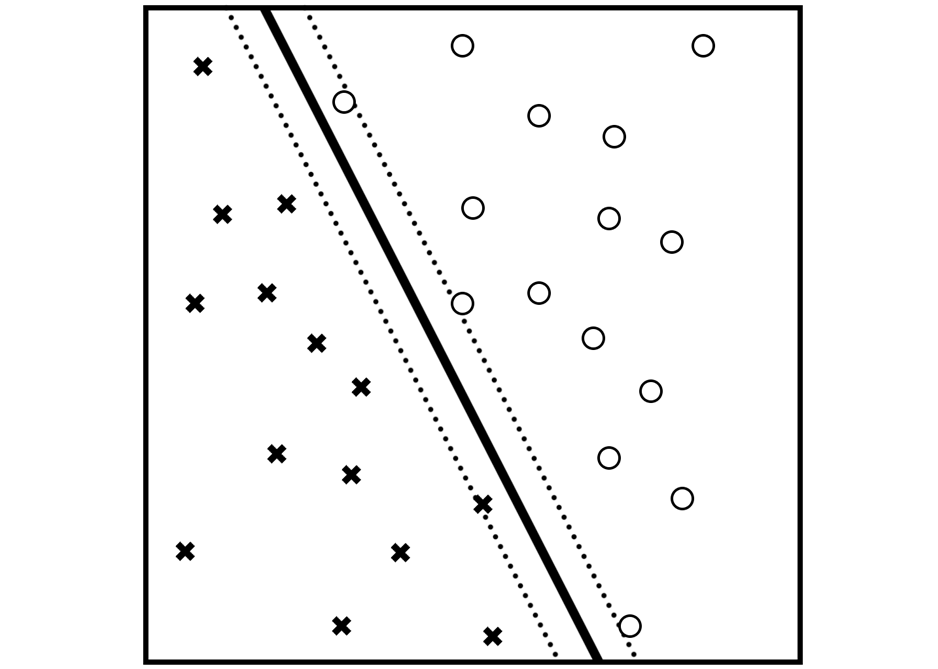
\includegraphics[width=\linewidth]{figures/svm}
  \captionof{figure}{An illustration of a machine learning algorithm learning to
    create a decision boundary between two ``concepts.''}
\end{Figure}

\noindent All on its own, an algorithm (such as \textit{decision trees}) can
emulate the creation of these internal concepts without any kind of target
data---i.e.\ without being told what to do with the input data.  Again, this
works because the algorithm can perform certain measurements on the data,
grouping or splitting it into segments that fit certain criteria.  This is
called unsupervised learning.  More relevant to this thesis, however, is
\textit{supervised} learning which is laid out in more detail below.

\subsection{Generalization}

Machine learning works by \textit{generalizing} problems, given specific input
data.  That is, generalization means that a machine learning algorithm, through
training, creates a model of the problem and learns to produce solutions for it.
If the model produces satisfactory solutions on previously unseen inputs, the
algorithm has created a generalized model of the problem.
\citet[p.~110]{Goodfellow-et-al-2016} correctly points generalization out as the main
area of concern in the field of machine learning:

\blockquote{
  \slshape%
  The central challenge in machine learning is that we must perform well on new,
  previously unseen inputs---not just those on which our model was trained. The
  ability to perform well on previously unobserved inputs is called
  generalization.
}

\subsection{Regression}

Regression, as opposed to classification (determining what discrete class a data
point belongs to), is used to estimate real-numbered variables from
relationships between dependent and independent variables.  That is, when a
problem has a solution that is not discrete (i.e.\ binary; yes/no, or trinary;
left, forward, right and so on) but rather, is real-numbered (e.g.\ temperature
or length), regression is used. An \textsc{ann} can be configured to handle both
problems of regression and classification by selecting the appropriate
activation function for the neural network's final layer.

\subsection{Supervised Learning}

Supervised learning means that a machine learning algorithm is trained by
providing it with \textit{target} data.  Explained more colloquially, it can be
understood as showing a toddler different objects and telling her what the
different objects are, over and over again until the toddler can identify the
different objects on her own.  Algorithmically, we are now talking about
\textit{artificial neural networks}, which, as the name implies, bears certain
similarities to the human brain.  Machine learning algorithms trained with
supervised learning can learn to identify a number of factors that are not
easily defined by logic systems.  Going back to the example with the stove
presented earlier; by presenting the \textsc{ann} with a temperature (and other
features relevant to identifying the correct answer) and telling it whether that
temperature is hot or not (as indicated by, for example, a human supervisor
making an informed decision), the \textsc{ann} eventually learns to model the
problem by modifying its internal state.

With enough training, the \textsc{ann} can then be presented with data and asked
whether the data represents a hot or a cold stove, making decisions very close
to the ones made by the supervisor during the learning phase.  Not only that,
but being presented with \textit{unseen} data, the \textsc{ann} will show an
ability to make a sane decision in regard to the data representing a hot stove
or a cold stove---the \textsc{ann} has learned to make decisions on its own, on
previously unseen data.

\subsection{Artificial Neural Networks}

Firstly, an artificial neural network has a hierarchical structure and uses a
learning algorithm for modeling a problem, a concept based on the biological
brain.  The algorithm is a simplistic abstraction of neural processing in the
mammalian central nervous sytem; a neuron is stimulated (a weight sum of input
values are fed into a neuron), the neuron is activated (the weighted sum is
passed through the activation function) and its output (activation) is relayed
to neighboring neurons (fed to neurons in the next layer).  Although artificial
neural networks can be configured in many different ways, all setups normally
consist of an input layer (a number of input nodes or neurons), one or more
hidden layers, and an output layer.

Training an \textsc{ann} consists of two major phases; the feed-forward phase
and the backpropagation phase.  During the feed-forward phase, weighted sums of
the inputs are forward-propagated through the network and passed through each
neuron's activation function.  At the end of the feed-forward phase, the output
error between the actual output and the true output is calculated, after which
the backpropagation phase begins.  During the backpropagation phase, the error
is backward-propagated through the network.  Lastly, the \textit{weights} (see
illustration below) are adjusted to reduce the error.

\begin{Figure}
  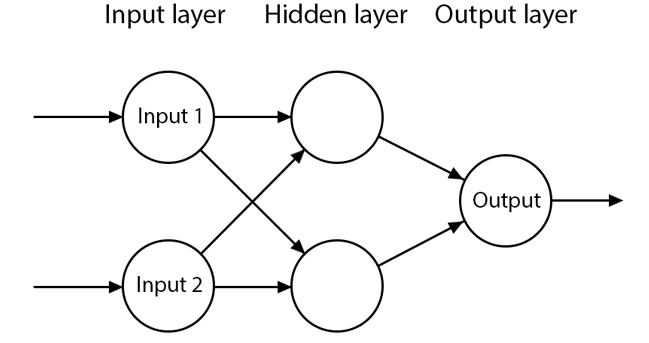
\includegraphics[width=\linewidth]{figures/ann}
  \captionof{figure}{A small \textsc{ann} with arrows between nodes
    representing the weights.}
\end{Figure}

\noindent An input value is fed to each input node and the resulting values are
multiplied by their respective weights---connection strengths to neurons in the
next layer (illustrated by the lines between cells in fig. 2.4 above)---added
together and then passed on as input values to nodes in the next layer in the
network.  For supervised learning---training the network by providing it with
target data---the output node values are then compared to the target data, an
error is calculated and the weights are adjusted accordingly.  On the next
iteration, the resulting output node values will be a little bit closer to the
target data.  The process is repeated until the network has reached a certain
level of proficiency in modeling the problem and providing accurate output
values.  The end result is a set of weights that gives the algorithm a way of
modeling the problem, thus producing \textit{correct} output for a given set of
inputs.

\subsubsection{The Feed-forward Phase}

First, input is fed to the \textit{input layer cells}. For the input layer,
these means that their final \textit{output values} are set to the data being
fed to the rest of network.

After that, the \textit{output} is calculated for each node or cell in
consecutive layers according to Equation~\ref{eq:node-activation} during the
\textit{feed-forward phase}:

\begin{Figure}
  \begin{align*}
    & \sigma(x) = \frac{1}{1+e^{-x}} \\
    & out_{c} = \sigma\left( \sum\limits_{p}
      \mathit{out_{p}} \cdot \mathit{weight_{p,c}}+\beta \right) \\
    & \text{where } p \text{ is a cell in the previous layer and } \\
    & \text{$\beta$ is the bias value from the previous layer.}
  \end{align*}
  \captionof{eqn}{\textsc{ann} cell output formula using the logistic
    function as the activation function.}
\label{eq:node-activation}
\end{Figure}

\noindent Or, in pseudocode:

\begin{Figure}
  \small
  \begin{algorithmic}
    \Function{get\_output}{$\mathit{c}$}
    \State${\mathit{net}}\gets 0$
    \For{$p$ in \textproc{previous\_layer} ($c$)}
    \State${\mathit{net}}\gets \mathit{net}+\textproc{get\_output}(p)\times
    \textproc{weight}(p, c)$
    \EndFor%
    \State$\mathit{out}\gets \textproc{activation}(\mathit{net}+\textproc{bias}(\textproc{previous\_layer}(c))$
    \State\Return{$\mathit{out}$}
    \EndFunction
  \end{algorithmic}
  \captionof{algo}{Pseudocode for calculating cell output in an \textsc{ann}.}
\end{Figure}

\noindent After this, the \textit{error} needs to be calculated.  This is done
by calculating the sum of squared errors\footnote{The sum of squared errors is
  one method of calculating the total error, used for the sake of communicating
  the theory of neural network internals.  It is not the only method viable for
  the purpose of calculating the total error value..} of the output neurons.
The goal is to minimize it (during the backpropagation phase), but first, it
needs to be calculated, which is done using Equation~\ref{ex:error-eqn}:

\begin{Figure}
  \begin{align*}
    & E_{total} = \frac{1}{2}\sum\limits_{o} {(\mathit{target_{o}-out_{o}})}^2 \\
    & \text{where } o \text{ is a cell in the output layer}
  \end{align*}
  \captionof{eqn}{Squared error calculation of an \textsc{ann} output.}
\label{ex:error-eqn}
\end{Figure}

\noindent At this point, the feed-forward phase is completed and an error
(deviation from \textit{target output}) has been calculated.  It is time to move
on to the backpropagation phase of the \textsc{ann} learning process.

\subsubsection{The Backpropagation Phase}

After the error has been calculated, it is \textit{propagated} back
throughout the \textsc{ann}, starting at the output nodes.  For each weight in
each layer, the \textit{gradient}---the partial derivative of the error function
with respect to each weight---is computed.  Using the value of the gradient, the
\textit{weight} is adjusted for each node.  The magnitude of the change to the
network's internal state for each learning iteration is dictated by a
\textit{learning rate}---a multiplicative variable dictating the rate of change
in the internal state.

For each node, the delta ($\delta$) value is computed for the output layer
neurons:

\begin{Figure}
  \begin{align*}
    \delta_o & =
      \frac{\partial E_{total}}{\partial \mathit{out_{o}}} \times
      \frac{\partial \mathit{out_{o}}}{\partial \mathit{net_{o}}} \\
           & =
      \frac{\partial E_{total}}{\partial \mathit{out_{o}}} \times
      \sigma'({net_{o}}) \\
    \text{where ${net_{o}}$} & \text{ is the weighted sum of all inputs to a} \\
    &\text{\hspace{-4.5em}node (logits).}
  \end{align*}
  \captionof{eqn}{Computing the $\delta$ value for an output neuron.}
\end{Figure}

\noindent Then, iterating through the layers backwards, all delta values are
computed:

\begin{Figure}
  \begin{align*}
    \delta_{c} & = \left(\sum\limits_{h} \delta_{h} \times
             \mathit{weight_{c,h}}\right) \times \sigma'(\mathit{net_{c}}) \\
    & \text{where } h \text{ is a cell in the }\textit{next}\text{ layer in
      the }\textsc{ann} \\
    & \text{and $c$ is the cell that the delta value is being} \\
    & \text{computed for.}
  \end{align*}
  \captionof{eqn}{Computing the $\delta$ value for a hidden layer neuron.}
\end{Figure}

\noindent After this, the computed delta values are used to adjust the
weights in the \textsc{ann} and the next activation of the model with the same
input data will produce a lower error value.

\subsection{Gradients}

As shown above, gradients---partial derivatives---are calculated during the
backpropagation phase to adjust the internal state into one that more aptly can
reproduce the supervised solution to the problem---the target data.  The
adjustment done to the weights is proportional to the gradient; a gradient of
larger magnitude means a larger adjustment made to the associated weight in the
\textsc{ann}s composition.

The \textit{chain rule} is applied to compute the gradient for each node
throughout the \textsc{ann} (starting at an output node or neuron):

\begin{Figure}
  \begin{align*}
    (f \circ g)' = (f' \circ g) \cdot g' = f'(g(x)) \cdot g'(x)
  \end{align*}
  \captionof{eqn}{The chain rule, used for computing gradients in the
    \textsc{ann}.}
\end{Figure}

\noindent That is; how much a weight in the \textsc{ann} needs to be adjusted is
dependent on its gradient with respect to each node going back to the output
node whose error is being minimized---the chain rule applied in sequence to each
neuron along the way.  For deeper \textsc{ann}s, this is not problem-free,
something that is discussed in the vanishing gradients section
below.

\subsection{Optimization}

The gradients described above can be optimized in different ways.  Not only are
there several different error functions (also called \textit{objective
  functions} or \textit{loss functions}), but there are also several different
methods for optimizing weights. The weight optimization function is called the
gradient descent optimization method.  This optimization method---not to be
confused with the error or objective function---is the method used for
minimizing the \textit{output} of the error function through an iterative
process (training).

\subsubsection{Stochastic gradient descent (\textsc{sgd})}

Perhaps the most basic of optimization methods, the Stochastic Gradient Descent
is an incremental gradient descent, finding a local minima or maximum through an
iterative process, where weights are adjusted little by little, repeatedly.

\subsubsection{Root-mean-square propagation (\textsc{rmsprop})}

The Root-Mean-Square Propagation is an improvement over the Stochastic Gradient
Descent.  Compared to the \textsc{sgd}, it introduces the concept of momentum,
maintaining a more direct route towards a local minima
\citep{tieleman2012lecture}.

\subsubsection{Adaptive moment estimation (\textsc{adam})}

Adaptive moment estimation---generally called Adam---is, in practice, a patched
version of the root-mean-square propagation method.  They are identical except
for the fact that Adam uses running averages of both the gradients as well as
their magnitudes \citep{kingma2014adam}.

\subsection{Overfitting}

If the \textsc{ann} is configured incorrectly in regard to the problem to be
solved, \textit{overfitting} can occur.  It can be intuitively understood
through visual representation (see below), but can also be described in the
following way: Overfitting occurs when the \textsc{ann} is too complex (i.e.\
consists of too many neurons, layers or a combination thereof) in regard to the
training data volume and/or problem complexity: The multi-dimensional polynomial
represented by the \textsc{ann}s internal state intersects every data point in
the training data---\textit{but}---inbetween the data points, it deviates from
the expected or reasonable positioning.  This renders the \textsc{ann} able to
solve any problem presented in the training data perfectly, but \textit{unable}
to solve any problem that it has not already encountered in the training data.
Overfitting can be solved by removing neurons from the network (i.e.\
simplifying the \textsc{ann} configuration) or providing a greater volume of
training data, which, in turn, fills up the spaces inbetween the previous
training set data points, preventing polynomial deviation.

\begin{Figure}
  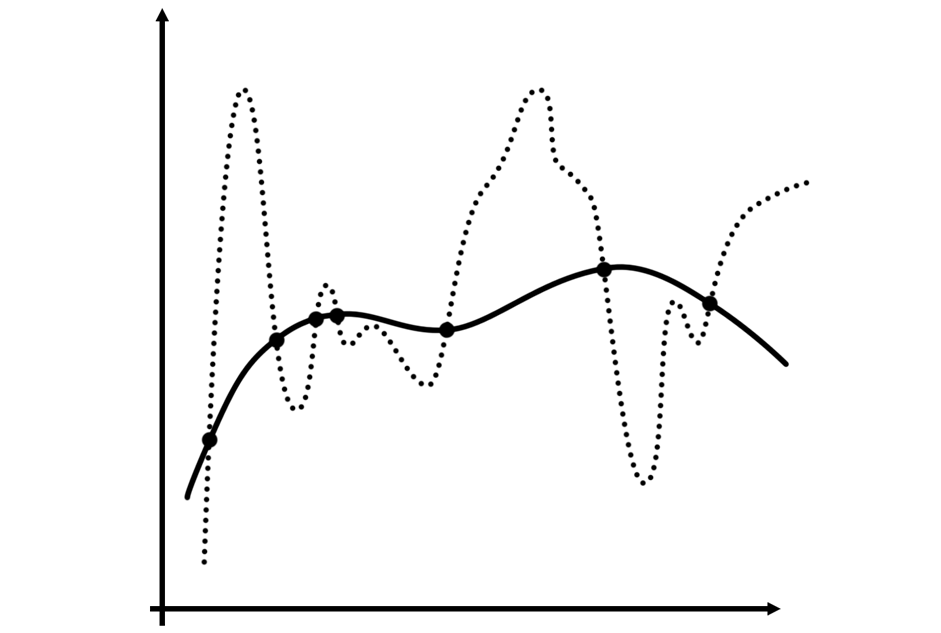
\includegraphics[width=\linewidth]{figures/overfit}
  \captionof{figure}{Overfitting---the solid curve is a more sane representation
    of the data points, compared to the dotted curve, which has been
    \textit{overfitted}.}
\end{Figure}

\noindent Another way of countering this problem is a method called
\textit{dropout} \citep{hinton2014}.  In effect, it does exactly what is
prescribed as a solution above; reducing the complexity of the \textsc{ann}.
However, it does this not by reconfiguring the network permanently, but by
\textit{randomly disabling nodes during training}.  That is, at the beginning of
a training iteration, a certain portion (called the \textit{dropout
  probability}) of the neurons is disabled, and the iteration is performed as if
the disabled neurons were not part of the model.  After the iteration has
completed fully, the neurons are re-enabled and another set of neurons are
selected randomly again to be disabled on the next training iteration.  Dropout
is only applied during training.

\subsection{Feature Extraction}

The extraction and selection of \textit{features} can be very important
depending on the problem.  Rather than feeding a neural network model raw input
data---data that has not been touched---which might work well depending on the
problem being solved, certain computations are performed on the input data to
create features.  Feature extraction involves performing computations on the
input data to create new features, making certain aspects of the input data more
prominent to the neural network model as well as reducing redundancy.  This, in
turn, reduces training time, allowing the \textsc{ann} to model the problem
faster as well as reducing overfitting \citep{bermingham2015application}.

On top of feature extraction, feature \textit{selection} is performed: Certain
features are kept while others are discarded from the input data.  For example,
when features are highly correlated with each other, only one of the features
might be kept, reducing the dimensionality, which also helps reduce training
time and model overfitting.

Another important aspect regarding features needs to be brought up; feature
\textit{scaling} (also called \textit{data normalization}).  Feature scaling is
a method used to standardize the \text{range} (i.e.\ $\mathit{feature_{min}}$ to
$\mathit{feature_{max}}$) of features.  For example, it is
unwanted for one feature to have a very large range, and another, independent
feature variable, to have a very small range.  The larger a range is compared to
other feature variable ranges, the more it will dictate the value of the error
function, causing the error function to ``focus'' more on the large range
features than on others, mistakingly ascribing the large range feature a greater
importance in the optimization process, which leads to a much slower convergence
of neural network weights.

All in all, feature extraction, selection and scaling play an important role in
optimizing neural network training for specific problem solving tasks.

\subsection{Recurrent Neural Networks}

A \textit{recurrent} neural network (\textsc{rnn}) is an artificial network that
is ``rolled out'' in the sense that connections between neurons form a
\textit{cycle}.  Essentially, what was understood as the \textit{depth} in the
\textsc{ann} is more akin to the \textit{width}---the length of the input
sequence---of the \textsc{rnn}.  While \textsc{rnn}s can also be deep, the
architecture of (deep) \textsc{rnn}s could be viewed as multiple \textsc{ann}s
stacked with lateral connections between layers.

The \textsc{rnn}, rather than merely outputting values forward through the
layers in the network (as does the \textsc{ann}), output values are also fed
back as inputs to previous layers, hence creating a feedback loop.  This creates
an internal state in the neural network---a short-term memory allowing
information to persist or linger---which takes into account previous input
values when processing newer ones.  In practice, this means that a single,
specific value can carry different meanings depending on previous inputs to the
\textsc{rnn}, or expressed in another way; that specific value can mean
something different depending on where, in the sequence of values, it is
encountered.  As a trivial example; in natural language, the same word carries
different meanings depending on where, in a sentence, it occurs.

Perhaps self-explanatory, this is why \textsc{rnn}s work well for time series;
each input affects the next iteration (essentially creating a \textit{memory}),
and so the order of the inputs becomes important, meaning that the \textsc{rnn}
takes entire sequences into account when modeling a problem rather than single
inputs.  It is not necessary for the data points in the sequence to be evenly
spaced in time, although that is the most common scenario depending on the
problem being modeled.

There are several different \textsc{rnn} architectures, some more known and used
than others.  Due to the nature of \textsc{rnn}s and the application of the
chain rule for calculating gradients, they have all been plagued by the
vanishing gradients problem.

\subsection{Vanishing Gradients}

It turns out that the gradient in multi-layer neural networks is unstable.  Not
only that; the stability decreases exponentially with depth (or, in the case of
\textsc{rnn}s, also sequence length).

As the chain rule is applied throughout the neural network---explained in the
description of the backpropagation phase earlier---the delta values comprise
a series of multiplications.  Continuing the use of the logistic function from
earlier in this example, the problem of vanishing gradients is easy to
understand.

As the maximum derivative of the logistic function is $\frac{1}{4}$, a long
series of multiplications throughout the nodes in the neural network converge to
zero.

\begin{Figure}
  \begin{align*}
    \sigma'(x) & = \frac{e^x}{{(1+e^x)}^2} \\
    \sigma'(0) & = \frac{1}{4}
  \end{align*}
  \captionof{eqn}{The derivative of the logistic function and its maximum
    value at $x=0$.}
\end{Figure}

\noindent In an \textsc{ann}, the depth (width or \textit{roll out} in the
\textsc{lstm}) dictates the length of the multiplication series: In the last
hidden layer, for example, the chain rule gives the following gradient
computation:

\begin{Figure}
  \begin{align*}
    \delta_{cell} & =
      \frac{\partial E_{total}}{\partial \mathit{out_{cell}}} \times
      \frac{\partial \mathit{out_{cell}}}{\partial \mathit{net_{cell}}} \\
                 & =
      \frac{\partial E_{total}}{\partial \mathit{out_{cell}}} \times
      \sigma'({net}_{cell}) \\
    \frac{\partial E_{total}}{\partial \mathit{weight_{cell}}} & =
      \delta_{cell} \times
      \frac{\partial \mathit{net_{cell}}}{\partial \mathit{weight_{cell}}}
  \end{align*}
  \captionof{eqn}{Gradient calculation formula.}
\end{Figure}

\noindent As the gradient is computed for cells farther upstream in the neural
network, the multiplication becomes longer and longer---more and more delta
values are multiplied together, resulting in a convergence ($\frac{1}{4}^n$
where $n$ is the number of cells along the path from the current node to the
output node, ignoring other multiplicative factors) towards zero in the limit.

\subsection{Long Short-Term Memory}

In 1997, Hochreiter and Schmidhuber introduced the Long Short-Term-Memory
(\textsc{lstm}).  Building upon the traditional \textsc{rnn}, they introduced
three \textit{gates} that manage the internal cell state: The input, output and
forget gates.

During training, these gates are used to decide how to adjust the internal state
to adapt it to the information being fed to the \textsc{lstm}.  For example, the
first step is to decide how much of the alread-existing internal cell state to
throw away.  This is managed by the forget gate.  Then, the input gate decides
which of the internal values to update, after which the internal state is
adjusted and adapted to the new information.  Lastly, the output gate decides
what the \textsc{lstm} will output.  Although this output is based on the
internal state, it is not the entire state---rather, how much of the internal
state, and what parts of the internal state, are output, is managed by the
output gate.

These gates work together to carefully protect the internal state from the
vanishing gradient problem---the forget gate can decide to ``turn off''
adjustments completely for many training iterations if they are not deemed
necessary by the \textsc{lstm}, which in turn reduces the problem and vastly
increases the information persistence in the internal state.

It should be noted, however, that the problem is not fundamentally solved, but
rather, its effect is reduced to the point of \textsc{lstm}-based \textsc{rnn}s
being \textit{much} more competent at modeling long-term temporal relationships
in the input sequences compared to traditional \textsc{rnn}s.

\subsection{Sequence-to-Sequence Learning}

Sequence-to-sequence learning implies that the network is being trained to
produce \textit{sequences} as output, from input sequences.  Rather than
producing a single output data point predicted to follow the input sequence, the
\textsc{lstm} produces an output \textit{sequence}, predicted as the sequence to
follow the provided input sequence.  For example, provided with a natural
language sentence of words, the entire following sentence (sequence of words)
would be predicted.  This approach is also used in machine translation
\citep{sutskever2014sequence}; an input sentence is provided, and an output
sentence is predicted in the foreign language.  For financial time series, this
implies feeding the \textsc{lstm} with a sequence of data points and training it
on the \textit{sequence} of data points following the input sequence.  That is,
the \textsc{lstm} is provided with (for example) five minutes of data as the
input sequence and the following next five minutes of data as the target data
sequence.  Sequence-to-sequence learning, thus, involves a many-to-many mapping
of the time series data.

\section{Algorithmic Trading}

Algorithmic trading (also known as algo-trading, automated trading and black-box
trading) is a way of automating trading by delegating market entry and exit
decisions to an algorithm (i.e.\ letting an algorithm decide when to buy, sell or
short a certain stock).

\subsection{Black-box Trading}

Although an algorithm is normally thought of as being constructed by human
reasoning with steps laid out in sequence, it should now be understood as a
machine learning algorithm learning to construct solutions to various
problems. The \textsc{ann} models the problem, emulating a way of reasoning
about it. Thus, algorithmic trading ties together the knowledge presented in the
theory chapter, building upon it to create a machine learning algorithm
attempting to understand aspects of financial market behavior.

The term \textit{black-box trading} hints at this; the intricacies of a trained
neural network cannot be understood (or, put in a simpler way, it is not known
why the \textsc{ann} takes certain decisions, and it cannot be known easily by
looking at the internal state of the \textsc{ann} without actually activating it
with some input data).  In practice, the internal state of the \textsc{ann}
represents an algorithm that produces a conclusion in regard to a presented
problem.

Despite this, it is expected that the \textsc{ann} models market behavior to
some extent to provide relevant output data.

Since algorithmic trading algorithms can be fully automated, under the right
circumstances (for example, low data transfer latency to the broker and a high
level of computational power together with an effective algorithm [in terms of
market behavior prediction performance]), returns could potentially be generated
arbitrarily quickly, though being limited by the available trading capital and
market liquidity.  This fact is backed up by real-world algorithmic trading
algorithms generating positive net returns, although most of these models are
trade secrets.

\subsection{Non-stationarity}

Machine learning algorithms, used in a trading scenario as explained above,
model the trading problem by relying on recurring patterns in the input data.
Due to non-stationarity, two identical financial time series input sequences
acquired at two different points in time may have different solutions (i.e.\
output sequence predictions).  Just as a human trader continously needs to adapt
to changing market conditions, an automated trading system also needs to
continously adapt its behavior.

This problem is a fact of complex time series and cannot be fully overcome, but
can be countered to some degree by, for example, using input time series from a
fairly short period of time if the neural model is not complex enough: The
market behavior today is vastly different compared to before the stock market
crash in 2008---just as human traders cannot use the same strategies today as
they used back in 2007, a machine learing trading algorithm trained on data from
that time period would have developed a strategy that does
not work in today's market. \\

--- Lastly, with all knowledge in the theory chapter in mind, the methodology
chapter and our particular experiments will become easily understandable, as
well as issues encountered during our research.
